\documentclass{article}

\usepackage{spconf,amsmath}
\usepackage{bm,bbm}
\usepackage[boxed]{algorithm2e}
\usepackage[caption=false,font=footnotesize]{subfig}
\usepackage[binary-units]{siunitx}
\usepackage{booktabs}
\usepackage{url}
\usepackage{graphicx}
\usepackage[numbers]{natbib}


\title{Transition Graphs for SAR Image Texture Characterization:\\ An Exploratory Study}

\name{Eduarda T.\ C.\ Chagas$^a$, Heitor S.\ Ramos$^a$, Osvaldo A.\ Rosso$^b$, and Alejandro C.\ Frery$^c$}
\address{
$^a$Departamento de Ci\^encia da Computa\c c\~ao, Universidade Federal de Minas Gerais, Brazil
\\
$^b$Instituto de F\'isica, Universidade Federal de Alagoas, Brazil
\\
$^c$School of Mathematics and Statistics, Victoria University of Wellington, New Zealand
}

\begin{document}
\maketitle

\begin{abstract}

%A new perspective on the analysis of surfaces and land use has been carried out with the synthetic aperture images (SAR) extraction and classification.
%With the popularization of the machine and deep learning techniques, such algorithms have revolutionized the performance and interpretability of their results~\cite{han2020unsupervised, huang2020classification, xie2020polsar}.

\citet{PermutationEntropyBandtPompe} proposed a nonparametric approach to time series analysis that has been used successfully applied in several scientific areas~\cite{baravalle2018discriminating, Araujo2019permutation, ClassificationVerificationOnlineHandwrittenSignatures}.
The Bandt-Pompe methodology consists of 
recording the observations' relative order in small subsets of the time series.
Two kinds of analyses follow: the patterns' marginal distribution, and their transitions~\cite{LearningandDistinguishingTimeSeriesDynamicsViaOrdinalPatternsTransitionGraphs2019,MultiscaleOrdinalNetworkAnalysisofHumanCardiacDynamics}.
The former stems from the histogram of such patterns, while the latter consists of estimating the stochastic matrix of the Markov chain that describes subsequent patterns.
Then (at least) two measures are computed: the Permutation Entropy (which quantifies the disorder) and a distance from the uniform distribution.
The Complexity of the process is the product of the Permutation Entropy and such a distance.
The time series is then mapped onto a location (point) in the Entropy-Complexity plane.
Such a location often reveals hidden characteristics, for instance structural differences between chaos and randomness~\cite{DistinguishingNoiseFromChaos,Rosso2007}.

%Obtaining a new representation of the time series through the ordinal patterns, the distributions resulting from the histogram of frequencies or the pattern transition graphs become less sensitive to outliers and do not assume any hypothesis about the nature of the data.
%Despite its simplicity, this method is robust to noise, has a low computational cost and 
%when used in conjunction with causal descriptors from the Information Theory, 
%it has shown good results in signals characterization and classification.

\citet{ChagasClassification2020} proposed an extension of this methodology for SAR images texture analysis.
First, the image patch is transformed from \mbox{2-D} into a \mbox{1-D} signal with a Hilbert-Peano curve~\cite{Lee1994Texture}.
This dimensionality reduction preserves relevant properties of spatial pixel correlation (since such a curve never maintains the same orientation for more than three consecutive points) with a low computational cost.

The main contribution is a new ordinal patterns transition graph: the Weighted Amplitude Transition Graph (WATG), which discriminates similar patterns with different intensity variations.
We then compute the stochastic matrix of the Markov chain that describes subsequent patterns, and scale the probabilities by the maximum absolute difference of the corresponding observations.
We obtain the Shannon Entropy as
\begin{equation}
	H(\mathbbm{P}) = -\frac{1}{\log D!} \sum_{\ell=1}^{D!^2} p_\ell \log p_\ell,
\end{equation}
where $D$ is the ordinal patterns dimension, and 
$$\mathbbm{P} = \{p_{(\widetilde\pi^D_1, \widetilde\pi^D_1)}, p_{(\widetilde\pi^D_1, \widetilde\pi^D_2)}, \dots, p_{(\widetilde\pi^D_{D!}, \widetilde\pi^D_{D!})} \} = \{p_1,\dots,p_{D!^2}\}$$
is the scaled probability distribution obtained from the patch.

Although very expressive, the Shannon Entropy is not able to describe all possible underlying dynamics.
To this aim, \citet{LopezRuiz1995} proposed using the disequilibrium  $Q$, a measure of how far $\mathbbm{P}$ is from an equilibrium or non-informative distribution $\mathbbm{U}$.
We calculate this descriptor as:
\begin{equation}
	Q'(\mathbbm{P}, \mathbbm{U}) = \sum_{\ell=1}^{D!^2} \Big(p_\ell \log\frac{p_\ell}{u_\ell} +
	u_\ell \log\frac{u_\ell}{p_\ell}
	\Big),
\end{equation}
then we normalize $Q = Q'/\max\{Q'\}$.
With this, the Statistical Complexity which measures the dependence structures among the elements is $C = HQ$.
We can then map a sequence at a point $(h, c)$, where the set of all possible points is the Entropy-Complexity plane $H \times C$.
Fig.~\ref{fig:Outline} outlines these steps.

\begin{figure*}
	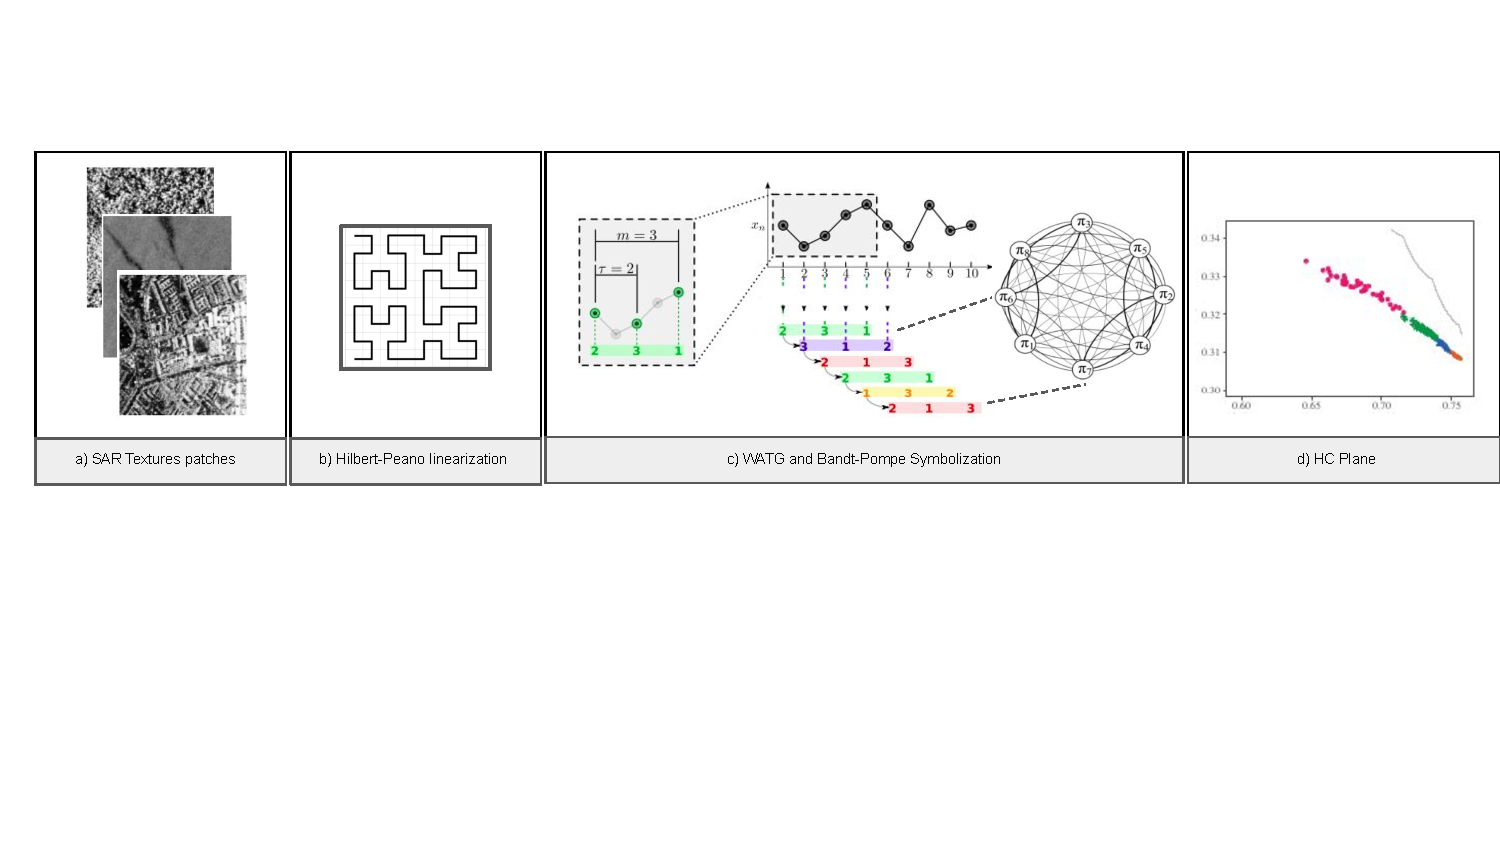
\includegraphics[width=\linewidth]{SARTexture.pdf}
	\caption{Outline of the methodology used for the textures classification.}
	\label{fig:Outline}
\end{figure*} 

\citet{ChagasClassification2020} showed that the WATG approach 
achieves a perfect separation between urban, pastures, ocean, and forest areas of UAVSAR images patches.
Additionally, this characterization has advantages over other approaches:
(i)~the features are easily visualized, and
(ii)~the training process of machine learning algorithms is fast and less costly.

The intensity and structure of SAR texture signals is directly related to the target's nature and backscattering properties.
Therefore, the WATG approach is a fruitful field of investigation.

In this context, we seek to analyze WATG in new scenarios for the classification of homogeneous textures, in which the following research questions stand out:
\begin{enumerate}
	\item What is the impact of patch size on the final descriptors?
	We obtained good results with patches of size $128 \times 128$.
	Thus, the objective of this experiment is to analyze the minimum dimension necessary to obtain good characterizations.
	
	\item How do the results vary with the polarization? 
	WATG was only applied to the HH-HH band of PolSAR quad images.
	We will investigate how the points in the $H\times C$ change when switching to other polarizations.
	
	\item How does the algorithm behave when exposed to different surfaces?
	We built a dataset with $700$ image patches of same dimension from  pasture, forest, oceans, glacial, desert, and urban regions.
	We will study the performance of WATG under mixtures of classes.
	
\end{enumerate}

\end{abstract}

\keywords{
Synthetic Aperture Radar (SAR), 
Terrain Classification,		
Information Theory, 
Ordinal Patterns.
}

\bibliographystyle{IEEEtranSN}
\bibliography{ref}

\end{document}